% EBMA paper for Political Analysis: As Accepted for Publication.



%\documentclass[pdftex,12pt,fullpage,oneside,endnotes]{amsart}
\documentclass[12pt,fullpage,endnotes]{article}
%\usepackage{apsr}
\usepackage{array,amsmath,psfrag,amssymb,subfigure,tabularx}
\usepackage{hyperref,multicol}
\usepackage{booktabs}
\usepackage[usenames]{color}
\usepackage{datetime}
\usepackage{dcolumn}
\usepackage{wrapfig}
\usepackage{setspace}
\usepackage{url}
\usepackage[english]{babel}
\usepackage{times}
\usepackage{multirow}
\usepackage[pdftex]{graphicx}
\usepackage{epstopdf}
\usepackage{lscape}
\usepackage{array}
\usepackage{booktabs}
\usepackage{hyperref}
\usepackage{endnotes}
\usepackage[top=2.54cm, bottom=2.54cm, left=2.54cm, right=2.54cm]{geometry} 
%\usepackage[nolist]{endfloat}

\newcommand{\note}[1]{\footnote{ #1 \vspace{4 mm}}}

\usepackage{natbib}
\bibpunct{(}{)}{;}{a}{}{,}
\bibdata{Bibliography_EBMA}
%\bibliographystyle{chicago}

\newboolean{blind}
\setboolean{blind}{false}


\title{Say Yes to the Guess: \\ Tailoring Elegant Ensembles on a Tight
  (Data) Budget\thanks{Presented at the 2012 Annual Meeting of the American Political Science Association, August 30 - September 2, New Orleans, Louisiana. 
%This work was partially supported by the Information Processing Technology Office of the Defense Advanced Research Projects Agency via a %holding grant to the Lockheed Martin Corporation, Contract FA8650-07-C-7749. The current support is partially from the Office of Naval %Research via ONR contract N00014-12-C-0066 to Lockheed Martin's Advanced Technology Laboratories.
    }}
\author{
Jacob M. Montgomery\\
	Department of Political Science\\
	Washington University in St. Louis\\
	Campus Box 1063, One Brookings Drive\\
	St. Louis, MO, USA, 63130-4899 
	\and
Florian M. Hollenbach  \\
	Department of Political Science\\
	Duke University\\
	Perkins Hall 326 Box 90204\\
	Durham, NC, USA, 27707-4330
	\and
Michael D. Ward\\
	Department of Political Science\\
	Duke University\\
	Perkins Hall 326 Box 90204\\
	Durham, NC, USA, 27707-4330\\
	corresponding author: michael.d.ward@duke.edu
} 




\date{\today}


\begin{document}

\maketitle
\thispagestyle{empty}
\clearpage
\pagestyle{myheadings}
\markright{Montgomery, Hollenbach, \& Ward\hfill Ensemble BMA\hfill}
\newpage
\singlespacing

\thispagestyle{empty}

{\centering \bf \large Say Yes to the Guess: \\ Tailoring Elegant Ensembles on a Tight (Data) Budget \\}

\begin{center}
\begin{tabular}{ccc}
Jacob M. Montgomery, & Florian Hollenbach, & \& Michael D. Ward\\
\end{tabular}
\end{center}

\begin{abstract}
  \noindent We consider ensemble Bayesian model averaging (EBMA) in
  the context of small-n prediction tasks with high rates of missing
  component forecasts.  With a large number of observations to
  calibrate ensembles and low rates of missing values for each
  component model, the standard approach to calibrating ensembles
  introduced by \cite{Raftery:2005} performs well. However, data in
  the social sciences generally do not fulfill these requirements. The
  number of outcomes being predicted tend to be relatively small and
  missing predictions are neither random nor rare. In these
  circumstances, EBMA models may overweight components with low rates
  of missingness and those that that perform well on the limited
  calibration sample.  This can seriously undermine the advantages of
  the ensemble approach to prediction.  We demonstrate this problem
  and provide a solution that diminishes these undesirable outcomes by
  introducing a ``wisdom of the crowds'' parameter to the standard
  EBMA framework. We show that this solution improves predictive
  accuracy of EBMA forecasts in both political and economic
  applications.  \today.
\end{abstract}

%\doublespacing
%\newpage


\setcounter{page}{1}

\section{Introduction}

Although accurate prediction of future events is not the primary goal
for most social sciences, recent years have witnessed spreading of
systematic forecasting from more traditional topics (e.g., GDP growth
and unemployment) to many new domains (e.g., elections and mass
killings) .  Several factors have motivated this increase.  To begin
with, testing systematic predictions about future events against
observed outcomes is generally seen as the most stringent validity
check of statistical and theoretical models.  In addition, forecasting
of important political, economic, and social events is of great
interest to policymakers and the public who are less interested in
testing theories of the world than correctly anticipating and altering
the future.

With the proliferation of forecasting efforts, however, comes a need
for sensible methods to aggregate and utilize the various scholarly
efforts.  One attractive solutions to this problem is to combine
prediction models and create an ensemble forecast.  Combining
forecasts reduces reliance on any single data source or methodology,
but also allows for the incorporation of more information than any one
model is likely to include in isolation.  Across subject domains,
scholars have shown ensemble predictions to be more accurate than any
individual component model and less likely to make dramatically
incorrect predictions \citep{Bates:1969,Armstrong:2001,Raftery:2005}.

The idea of ensemble learning itself has a long history in the machine
learning and nonparametric statistics community \citep{Hastie:2009}. A
wide range of statistical approaches including neural nets, bagging,
random forests, additive regression trees, and boosting and more may
be properly considered ensemble approaches.

One such method advocated recently for forecasting is ensemble
Bayesian model averaging (EBMA). This method was first proposed by
\citet{Raftery:2005} to improve weather forecasts.  It has recently
been suggested as a useful method for the social sciences by
\citet{mhw:2012}. In essence, EBMA creates a finite mixture model that
generates a weighted predictive probability density function (PDF).
EBMA mixture models seek to collate the good parts of existing
forecasting models, while avoiding over-fitting to past observations
or over-estimating our certainty about the future.  The hope is for
greater accuracy as both the knowledge and implied uncertainty of a
variety of approaches are integrated into a combined predictive PDF.

However, there are several challenges for creating ensemble
predictions for many application in the social sciences.  To begin
with, the amount and quality of data for calibrating ensembles is far
from ideal.  EBMA was first developed for use in weather forecasting
where measurement of outcomes is fairly precise and data is relatively
abundant.  Predicting, for instance, water surface temperatures in 200
locations across five days provides 1,000 observations by which model
weights can be calibrated.  Forecasting quarterly GDP growth in the
United States for five \textit{years} provides only 20.

A second, and related, issue is dimensionality. Many prediction tasks
involve many more forecasts than observations.  For example, the well
known forecaster of U.S. politics, Nate Silver, updates his forecasts
of the 2012 presidential election weekly, yielding dozens of forecasts
for a single outcome \url{http://fivethirtyeight.blogs.nytimes.com/}.
Similarly, in the field of economics, a wide variety of consulting
firms, banks, and international organizations each provide multiple
forecast for various economic quantities. An example are the various
forecasts of the Federal Open Market Committee (FOMC) of the
U.S. Federal Reserve Board, which are frequently updated, as for
example here: \url{http://1.usa.gov/zjyisV}.

An additional issue is the inconsistency with which forecasts are
issued. Given the lengthy time periods involved, there are likely to
be many missing forecasts in any given time window.  Moreover, we
cannot assume that forecasts for any time period from a specific model
or team are missing at random.  Particularly unsuccessful forecasts
may be suppressed and some forecasting efforts are only active for
short time-periods due to poor performance.  Moreover, forecasts have
tended to accumulate with more potential components being available
for more proximate time periods. 

One example of forecasting that combines all of these issues in the
prediction of U.S. Presidential elections.  Table 1 represents nearly
the entirety of scholarly forecasts which produced more than one
out-of-sample forecast for elections in the 20th century.\footnote{
  See, for example \citet[][]{Fair:2009, Fair2011, Abramowitz:2008,
    Campbell:2008, Cuzan:2004,Cuzan:Bundrick:2008,hibbs:2012, Lockerbie:2008, Erikson:Wlezien:2008,
    Graefe:2010, Holbrook:2008}.  A recent symposium in {\em PS:
    Political Science \& Politics} presents and summarizes attempts by
  a variety of scholars to predict the 2012 U.S. presidential
  election. In the symposium contribution, we use the in-sample fitted
  values of the election forecasting models to calibrate the EBMA
  model. However, the strength of EBMA is greatest when the model is
  calibrated on true out-of-sample forecasts, thus we focus on these
  here.}  In this instance, we have only five observations by which
to calibrate an ensemble model, while we have nine forecasting models.
Moreover, several of the individual forecasts are missing for a
significant portion of the data.  The forecast of Cuz\`an, for
instance, is missing for 60\% of the elections in this
dataset.\footnote{The predictions by Cuz\`an for 2004 stems from the
  FISCAL model published prior to the 2004 election by
  \citet{Cuzan:2004}, while the 2008 prediction comes from the FPRIME
  short model presented in advance of the election
  \citep{Cuzan:Bundrick:2008}. However, both models are quite similar
  in their composition.}

\begin{table}[ht]
\caption{Pre-election forecasts of the percent of the two-party vote going to the incumbent party in U.S. Presidential elections}
\label{tab:one}
\footnotesize
\begin{center}
\begin{tabular}{rlrrrrrrrrr}
  \toprule
  & F & A & C & H & LBRT & L & Hol & EW & Cuz \\ 
  \midrule
  1992 & 55.7 & 46.3 & 49.7 & 48.9 & 47.3 &  &  &  &  \\ 
  1996 & 49.5 & 57.0 & 55.5 & 53.5 & 53.3 &  & 57.2 & 55.6 &  \\ 
  2000 & 50.8 & 53.2 & 52.8 & 54.8 & 55.4 & 60.3 & 60.3 & 55.2 &  \\ 
  2004 & 57.5 & 53.7 & 52.8 & 53.2 & 49.9 & 57.6 & 55.8 & 52.9 & 51.1 \\ 
  2008 & 48.1 & 45.7 & 52.7 & 48.5 & 43.4 & 41.8 & 44.3 & 47.8 & 48.1 \\ 
  \bottomrule

\end{tabular}
\end{center}
Forecasts were published prior to each election by \textbf{F}air, \textbf{A}bramowitz, \textbf{C}ampbell, \textbf{H}ibbs, \textbf{L}ewis-\textbf{B}eck and \textbf{R}ice (1992), Lewis-Beck and \textbf{T}ien  (1996-2008),   \textbf{L}ockerbie, \textbf{Hol}brook, \textbf{E}rikson and \textbf{W}lezien and \textbf{Cuz}\`an and Bundrick.  Data were taken from the collation presented at \url{http://fivethirtyeight.blogs.nytimes.com/2012/03/26/models-based-on-fundamentals-have-failed-at-predicting-presidential-elections/}.
\end{table}

While particularly egregious for presidential election forecasting,
these data issues are endemic to the social sciences.  In this manuscript,
we explore several adjustments to the basic EBMA model as specified in
\citet{mhw:2012} that can help applied researchers create ensemble
forecasts even in the presence of these data-quality issues.
Specifically, we show EBMA can be adjusted to easily accommodate
missing forecasts as first proposed by \citep{Fraley:2010}.  In
addition, we propose an alteration to the basic model to ensure that
no one component is overweighted due to strong performance in the
limited calibration period.  Below, we first introduce the basic EBMA
model in Section \ref{model}.  We outline modifications to the model
for missing-ness and small samples in Sections \ref{missing} and
\ref{woc}. In Section \ref{empirics}, we apply the adjusted EBMA model
to unemployment data as well as the presidential election forecasts
shown in Table~\ref{tab:one}.


\section{Notation and basic EBMA model} 
\label{model}

Assume a quantity of interest to forecast, $\mathbf{y}^{t^*}$, in some
future period $t^\ast \in T^\ast$.  Further assume that we have extant
forecasts for events $\mathbf{y}^t$ for some past period $t \in T$
that were generated from $K$ forecasting models or teams, $M_1, M_2,
\ldots, M_K$, for which have a prior probability distribution $M_k\sim
\pi(M_k)$. The PDF for $\mathbf{y}^t$ is denoted
$p(\mathbf{y}^t|M_k)$.  Under this model, the predictive PDF for the
quantity of interest is $p(\mathbf{y}^{t^*}|M_k$), the conditional
probability for each model is $p(M_k|\mathbf{y}^t) =
p(\mathbf{y}^t|M_k)\pi(M_k)/\underset{k=1}{\overset{K}{\sum}}p(\mathbf{y}^t|M_k)\pi(M_k)$,
and the marginal predictive PDF is $p(\mathbf{y}^{t^*}) =
\underset{k=1}{\overset{K}{\sum}}
p(\mathbf{y}^{t^*}|M_k)p(M_k|\mathbf{y}^{t})$.  This can be
viewed as the weighted average of the component PDFs where the weights
are determined by each model's performance within the already-observed
period $T$.

\subsection{Dynamic ensemble forecasting}

The EBMA procedure assumes $K$ forecasting models throughout the training
($T^{\prime}$) calibration ($T$) and test ($T^\ast$) periods. The
component models are calibrated in the training period
$T^\prime$. Optimally, the component model predictions for the
calibration period T are created out-of-sample. The goal is to estimate
the parameters for the ensemble prediction model using
$\mathbf{f}^{t}_k$ for period $T$.  It is then possible to generate
true ensemble forecasts ($\mathbf{f}_k^{t^\ast}$) for observations in
the test period $t^\ast \in T^*$.

Let $g_k(\mathbf{y}|\mathbf{f}_k^{s|t, t^\ast})$ represent the
predictive PDF of component $k$, which may be the original prediction
from the forecast model or the bias-corrected forecast.  The EBMA PDF
is a finite mixture of the $K$ component PDFs, denoted
$p(\mathbf{y}|\mathbf{f}_1^{s|t}, \ldots,
\mathbf{f}_K^{s|t})=\overset{K}{\underset{k=1}{\sum}} w_k
g_k(\mathbf{y}|\mathbf{f}_k^{s|t})$, where $w_k \in [0,1]$ are model
probabilities, $p(M_k|\mathbf{y}^t)$, and $\sum_{k=1}^Kw_k=1$. The
ensemble predictive PDF with this notation is then
$p(y|f_{1}^{t^\ast}, \ldots,
f_{K}^{t^\ast})=\overset{K}{\underset{k=1}{\sum}} w_k
g_k(y|f_{k}^{t^*})$.

Past applications have statistically post-processed the predictions for
out-of-sample bias reduction and treated these adjusted predictions as a
component model. \citet{Raftery:2005} propose approximating the
conditional PDF as a normal distribution centered at a linear
transformation of the individual forecast,
$g_k(\mathbf{y}|\mathbf{f}_k^{s|t}) = N(a_{k0} +
a_{k1}\mathbf{f}_k^{t}, \sigma^2)$. However, in the presence of sparse
data, including the additional $\mathbf{a}$ parameters risks
over-fitting and reduced predictive performance.  We therefore use a
simpler formulation where $g_k(\mathbf{y}|\mathbf{f}_k^{t}) =
N(\mathbf{f}_k^{t}, \sigma^2)$.  Thus, the ultimate predictive
distribution for some observation $y^{t^\ast}$ is 

\begin{equation}
\label{pdf}p(y|f_1^{s|t^\ast},
\ldots, f_K^{s|t^\ast}) = \overset{K}{\underset{k=1}{\sum}} w_k
N(f_k^{t^\ast}, \sigma^2).
\end{equation}

\noindent This, is a weighted mixture of $K$ normal distributions each with 
means  determined by $\mathbf{f}^{t^\ast}$ and scaled by the
model weights $\mathbf{w}$.

\subsection{Parameter estimation}

Since the component model forecasts, $f^t_1, \ldots, f^t_k$, are
pre-determined, the EBMA model is fully specified by estimating model
weights, $w_1, \ldots, w_k$ and the common variance parameter
$\sigma^2$.  We estimate these using maximum likelihood methods
\citep{Raftery:2005}, although \citet{Vrugt:2008} have proposed
estimation via Markov chain Monte Carlo methods.  The log likelihood
function is

\begin{equation}
\mathcal{L}(w_1, \ldots, w_k, \sigma^2)=\sum_tlog\left(\sum_{k=1}^Kw_kN(f^t_k, \sigma^2) \right).
\end{equation}


\noindent The log-likelihood cannot be maximized analytically, so
\citet{Raftery:2005} propose an EM algorithm which explicitly
expresses EBMA as a finite mixture model
\citep{mclachlan:peel:2000,imai:tingley:2012}.  We introduce the
unobserved quantities $z_k^t$, which represents the probability that
observation $y^t$ is ``best'' predicted by model $k$.  The E step
involves calculating estimates for these unobserved quantities using
the formula
\begin{equation}
\label{E-step}
\hat{z}^{(j+1)t}_{k} = \frac{\hat{w}^{(j)}_k
p^{(j)}(y|f_{k}^{t})}{\overset{K}{\underset{k=1}{\sum}}\hat{w}^{(j)}_kp^{(j)}(y|f_{k}^{t})},
\end{equation}
\noindent where the superscript $j$ refers to the $j$th iteration of
the EM algorithm.

Note that $w_k^{(j)}$ is the estimate of $w_k$ in the $j$th iteration and
$p^{(j)}(.)$ is shown in \eqref{pdf}.  Assuming these estimates of
$z_{k}^{s|t}$ are correct, it is then straightforward to derive the
maximizing value for the model weights. Thus, the M step estimates
these as 

\begin{equation}
\label{M-step}
\hat{w}^{(j+1)}_k=\frac{1}{n}\underset{t}{\sum}\hat{z}^{(j+1)t}_{k},
\end{equation}

\noindent where $n$ represents the number of observations in the
calibration dataset.  Finally,

\begin{equation}
\label{sigma}
\hat{\sigma}^{2(j+1)}=\frac{1}{n}\underset{t}{\sum}\overset{K}{\underset{k=1}{\sum}}\hat{z}^{(j+1)t}_{k}(y-f_{k}^{t})^2.
\end{equation}
\noindent The E and M steps are iterated until the improvement in the
log-likelihood is no larger than some pre-defined tolerance.  We
initiate the algorithm with the assumption that all models are equally
likely, $w_k = \frac{1}{K} ~ \forall ~ k \in [1, \ldots, K]$ and
$\sigma^2=1$.


\section{Missing forecasts}
\label{missing}
The above method, however, requires all component models to make
predictions for all observations in the calibration period. Thus, if
one model's observation is missing at time $t$, the only solution is
listwise deletion. To better accommodate missing values in component
models prediction within the EBMA procedure we follow
\citet{Fraley:2010} and modify the EM algorithm as
follows.\footnote{In future research, we intend to compare alternative
  methods for handling missing data. %, including the use of Gaussian
%  copulas to impute the missing predictions \citep{Hoff:2007}.
}
Define $$\mathcal{A}^t = \{i|\mbox{ensemble member i available at time
  t}\},$$\noindent which is simply the indicators of the list of
components that provide forecasts for observation $y^t$.  For
convenience, define $\tilde{z}_k^{(j+1)t} \equiv {{\underset{k \in
      A^t}{\sum}}\hat{w}^{(j)}_kp^{(j)}(y|f_{k}^{t})}/{\underset{k \in
    A^t}\sum w_k^{(j)}}$.  Equation \ref{E-step} above is then
replaced with

\begin{equation}
\hat{z}^{(j+1)t}_{k} = \Bigg\{ \begin{array}{c} {\hat{w}^{(j)}_k p^{(j)}(y|f_{k}^{t})}/{\tilde{z}_k^{(j+1)t} } \mbox{ if } k \in \mathcal{A}^t\\ 0 \mbox{ if } k \notin \mathcal{A}^t \end{array}
\end{equation}



\noindent  The M steps in Equations \ref{M-step} and \ref{sigma} are likewise replaced with

\begin{equation}
\hat{w}^{(j+1)}_k=\frac{\underset{t}{\sum}\hat{z}^{(j+1)t}_{k}}{\underset{t}{\sum}\overset{K}{\underset{k=1}{ \sum}} \hat{z}_k^{(j+1)t}}
\end{equation}


\noindent and

\begin{equation}
\hat{\sigma}^{2(j+1)}=\frac{\underset{t}{\sum}\overset{K}{\underset{k=1}{\sum}}\hat{z}^{(j+1)t}_{k}(y-f_{k}^{t})^2 }{\underset{t}{\sum}\overset{K}{\underset{k=1}{ \sum}} \hat{z}_k^{(j+1)t}}.
\end{equation}

\noindent In essence, the likelihood is renormalized given the missing
ensemble observations prior to maximization. Using the adjustments
above, the EBMA algorithm now allows for missing observations in the
component predictions.

%\section{Window selection} Jacob thinks this should be a short subsection eventually.  But not for APSA.

\section{Small sample adjustment}
\label{woc}

When ensembles are calibrated on very few observations, there is an
increased chance that EBMA may over-weight high performing models in a
way that reduces out-of-sample performance. This is especially true
when the short calibration period is combined with missing
observations in component model
predictions. %% We should probably do some simulations to show this.

To deal with this issue, we introduce a ``wisdom of crowds''
parameter, $c \in [0,1]$, that reflects our prior belief that all
models should receive some, but not necessarily equal, weight. We rescale $z^t_k$ to
have a minimum value $\frac{c}{K}$.  This states that there is, at a
minimum, a $\frac{c}{K}$ probability that observation $t$ is correctly
represented by each model $k$.  Since
$\overset{K}{\underset{k=1}{\sum}} z_k^t = 1$, this implies that
$z_k^t \in [\frac{c}{K}, (1-c)]$.  To achieve this, we replace
Equation \ref{M-step} above with

\begin{equation}
\hat{z}^{(j+1)t}_{k} = \frac{c}{K} + (1-c)\frac{\hat{w}^{(j)}_k
p^{(j)}(y|f_{k}^{t})}{\overset{K}{\underset{k=1}{\sum}}\hat{w}^{(j)}_kp^{(j)}(y|f_{k}^{t})}.
\end{equation}

Note that when $c=1$, all models are considered equally informative
about the outcome and $w_k=\frac{1}{K} \forall K$. Thus, we see that
the arithmetic mean or median of component forecasts for time period
$t$ represents a special case of EBMA where $c=1$.\footnote{The mean
  or median would be equivalent depending on if the posterior mean or
  median is used to make a point prediction.}  Likewise, the general
EBMA discussed in \citet{mhw:2012} represents a special case of this
more general model where $c=0$.

%\section{Simulations} Jacob thinks we will want just a bit of this.  But not for APSA.
% I agree. Twice.

\section{Applications}
\label{empirics}

%Generally, forecasting is not well developed or extensive in the social sciences.

We now turn to examining how these methods work in two areas that
exemplify forecasting in the social sciences. The first  is the estimation of  unemployment, 
and the second in the area of predicting the vote for the incumbent party in U.S. presidential
elections. Both areas have well developed forecasting traditions in the scholarly and policy community.


\subsection{Quarterly unemployment in the United States}
\label{econ}

Forecasting macroeconomic variables is a quite common exercise in the
field of economics and statistics. Calculating accurate forecasts of
economic variables is a necessity for policy makers and
businesses. These forecasts are created using a wide variety of
statistical models.\footnote{For a more comprehensive overview on
  foresting of economic variables and time-series forecasting see
  \citet{Elliott:Timmermann:2008} and \citet{Goijer:Hyndman:2006}.}
The majority of scholars employ time-series models, with the most
commonly applied statistical method being autoregressive integrated
moving average (ARIMA) and vector autoregressive (VAR) models. The
sophistication and complexity of forecasting models has increased
considerably over time. In particular, non-linear dynamic models have
gained prominence including threshold autoregressive models, Markov
switching autoregressive models and smooth transition autoregression
\citep{Elliott:Timmermann:2008,Montgomery:etal:1998}. More recently,
forecasters have introduced Bayesian VAR models and state-space models
to their arsenal \citep{Goijer:Hyndman:2006,Elliott:Timmermann:2008}.

Unsurprisingly, given the large number of ongoing forecasts, scholars
have attempted to improve predictive accuracy by combining forecasts
\citep{Bates:1969, Palm:Zellner:1992, Elliott:Timmermann:2008}.
Recently, EBMA and related Bayesian model averaging methods have been
successfully employed to create ensemble forecasts of various
macroeconomic indicators including inflation
\citep{Koop:2010,Wright:2009}, GDP \citep{Billio:2010}, stock prices
\citep{Billio:2011}, and exchange rates \citep{Wright:2008}.

Policy makers too have come to rely on ensemble forecasts of a sort.
The desire to aggregate the collective wisdom of multiple forecasting
teams is apparent in the \textit{Survey of Professional Forecasters
  (SPF)} published by the \textit{Federal Reserve Bank of
  Philadelphia}.  The \textit{SPF} includes forecasts for a large
number of macroeconomic variables in the U.S., including the
unemployment rate, inflation, and GDP growth.\footnote{The
  \textit{SPF} was first administered in 1968 by the American
  Statistical Association and the National Bureau of Economic Research
  (NBER).  Since 1990, however, it is run by the Federal
  Reserve Bank of Philadelphia.
  \url{http://www.phil.frb.org/research-and-data/real-time-center/survey-of-professional-forecasters/}}
In the first month of every quarter, a survey is sent to selected
forecasters and is returned by the middle of the second month of the
quarter. Forecasts are made for the current quarter as well as several
quarters into the future.

This plethora of predictions seems ideal for applying EBMA.  Nonetheless,
it is plagued by the same issues as discussed for the presidential
election forecasts shown in Table 1.  Even for quarterly measures,
there are relatively few observations, many forecasting teams, and a
significant number of missing observations.  This setting, therefore,
provides a test bed for the adjusted EBMA model discussed
above.

Here we focus on forecasting the civilian unemployment rate (UNEMP) as
published by the \textit{SPF}. For this application, we selected the
forecast horizon to be four quarters into the future, i.e. predictions
made in the first quarter of 2002 are for the first quarter of 2003
and so on. In total, the \textit{SPF} data on unemployment contains
forecasts by 569 different teams. However, for any quarter, the
average number of forecast teams making a prediction for four quarters
into the future is quite small and the majority of observations for
any given quarter are missing.\footnote{On average only 8.4 per cent
  of all teams make a forecast for any one quarter.}

To provide a meaningful benchmark, we also include the ``Green Book''
forecasts produced by the Federal Reserve. These forecasts are made by
the research staff of the Board of Governors and are handed out prior
to meetings of the Federal Reserve Open Market Committee
(FOMC).\footnote{One issue with forecast evaluation in many domains in economics is that the macroeconomic data (i.e. our ``true observations'') are revised regularly. The unemployment rate for a given quarter at that time is generally an estimate that is subject to revision when better data becomes available. When evaluating forecasts, it is thus important whether predictions are compared to the outcome data for each quarter available at the time or whether the revised and most recent data is used. As \citet{Croushore:Stark:2001}
  describe, depending on the forecast exercise, it can make a
  difference whether the forecast models are evaluated using
  ``real-time'' (original estimate) or the ``latest available'' (revised) data. We have decided here
  to use the ``latest available'' data and do not believe that it
  should make a difference in our case, as all predictions are
  evaluated against the same data and EBMA is a mixture of the
  component forecast models. Thus the component models and our benchmark model are estimated and evaluated on the same data. However, in a future version of this
  paper we will replicate this analysis using real-time data to
  evaluate the forecasts.} % Better now?

Taking the \textit{SPF} and Green Book unemployment forecasts, we
calibrate an ensemble model for each period $t$, using forecaster
performance over the past ten quarters.  Only forecasts that had made
predictions for five of these quarters were included in the ensemble.
Thus, the EBMA model uses only 163 models out of a possible 293
forecasting models that made predictions during the period we study.
Due to missing data early in the time series, and the fact that Green
Book forecasts are sequestered for five years, we generate forecasts
beginning in the third quarter of 1983 and running through the fourth
quarter of 2007.



\begin{figure}[h]
  \caption{Ensemble weights for SPF forecasts of U.S. unemployment
    with a rolling calibration window}
\label{modelWeights}
\begin{center}
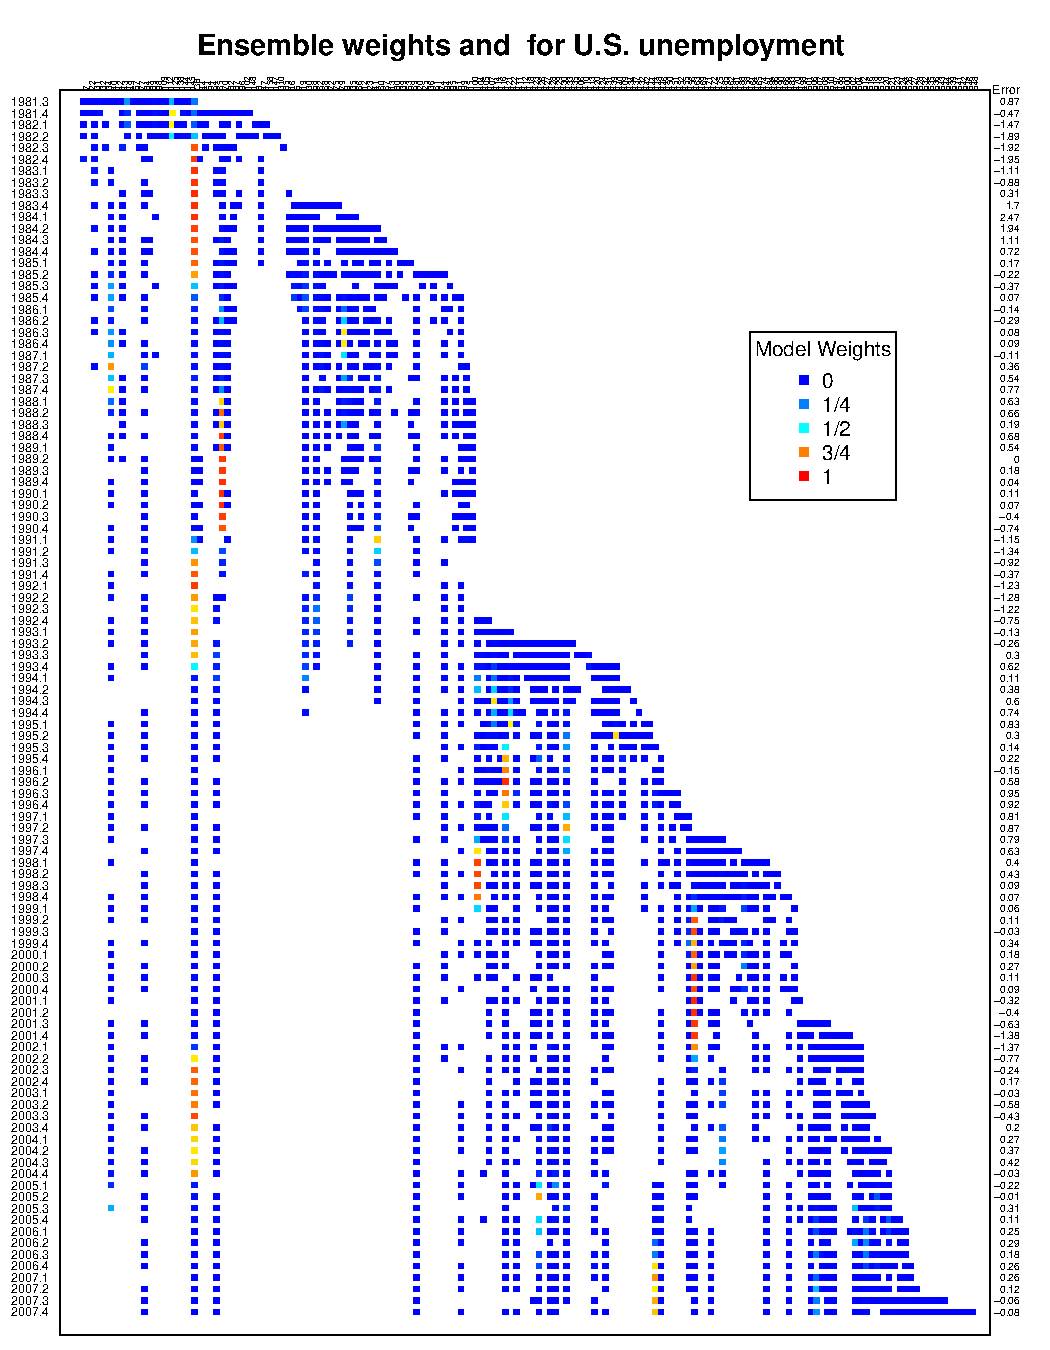
\includegraphics[scale=.90]{awesome}
\end{center}

\footnotesize This figure shows the component weights for each EBMA
model estimated between 1983 and 2007. Ensembles are calibrated on the
past ten quarters. The colors going from blue to red indicate
increasing weights for components in a given ensemble model. Those
components excluded in a given model are left blank.

\end{figure}

Figure \ref{modelWeights} provides a visual representation of EBMA
model calibrations throughout this period.  In this figure, the wisdom
of crowds tuning parameter is set to a modest $c=0.05$.  The colors
indicate the model weight assigned to each component on a red-blue
color ramp (components not included in the ensemble are blank).
Models assigned no weight are shown in dark blue while models that are
heavily weighted are shown in red. Figure \ref{modelWeights} also illustrates
the difficulties inherent in
forecasting with this type of data.  For any given year, only a subset
of forecasting teams offer a prediction.  Further, an even smaller
subset contains models that both offer a prediction and have made a
sufficiently large number of prior forecasts to facilitate model
calibration.  Finally, the very sparseness of the data encourages the
ensemble model to place a very large amount of weight on the best
performing models.  

We now turn to evaluating the performance of the ensemble relative to
its 163 component forecasts.  To do this, we focus on eight model fit
indices available in the literature.  The eight metrics we use are
mean absolute error (MAE), root mean squared error (RMSE), median
absolute deviation (MAD), root mean squared logarithmic error (RMSLE),
mean absolute percentage error (MAPE), median absolute percentage
error (MEAPE), median relative absolute error (MRAE) and percent worse
(PW).  The latter two metrics are measured relative to a naive model,
simply predicting the future rate of unemployment as being the same as
the current rate of unemployment.  Further details for these metrics
are shown in the Appendix \citep{brandt:freeman:schrodt:2011}.


\begin{figure}[h]
\caption{Comparing predictive accuracy of EBMA and component models with eight metrics}
\label{compare2Components}
\begin{center}
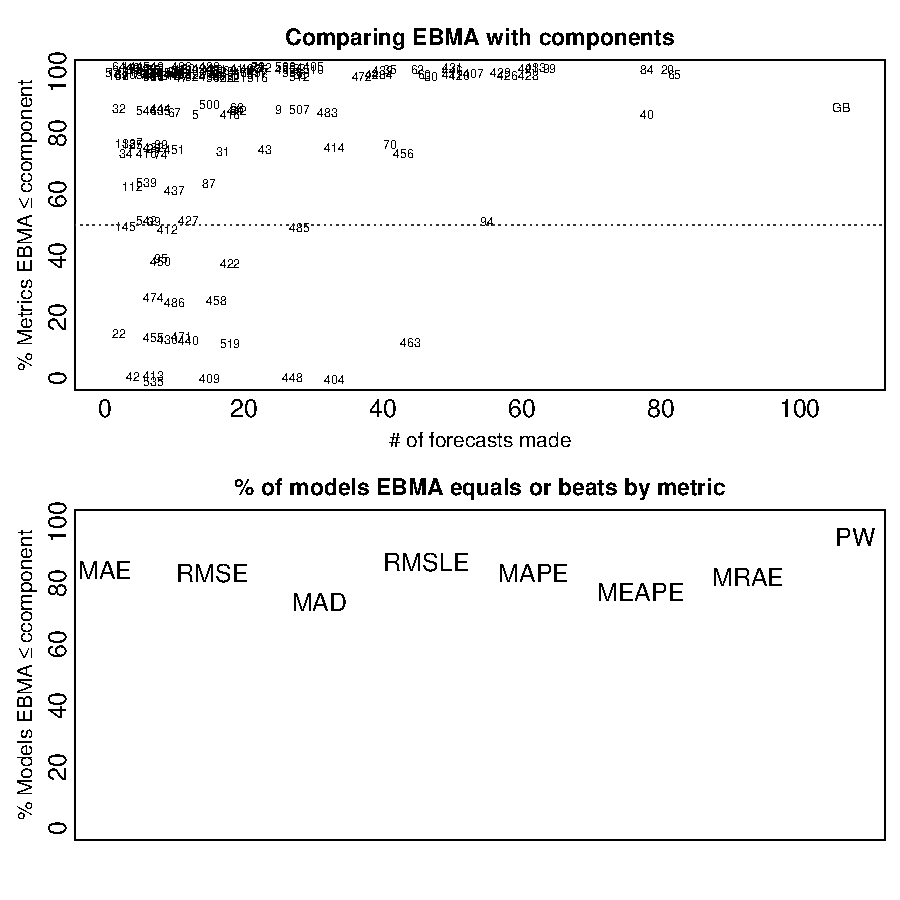
\includegraphics{compare2Components}
\end{center}

The top panel plots EBMA's relative performance, as measured by eight
forecasting metrics, to each of its components against the number of
forecasts generated by the component models.  The bottom panel shows
the percentage of component models that EBMA matches or outperforms as
measured by each metric.  Details on the eight forecasting metrics are
shown in the Appendix.


\end{figure}

It is important to note that many of these forecasters make
predictions in a relatively small subset of cases.  That is, each
model $k$ offers forecasts for only a subset of cases $n_k \subset n$.
To create a fair comparison, therefore, we calculate these fit indices
only for $n_k \forall k \in [1,K]$.  By this measure, the EBMA model
performs very well.  Figure \ref{compare2Components} provides a
summary of these results.  The top panel shows the percentage of
metrics by which EBMA outperforms each component. The bottom panel
shows the percentage of component models that EBMA ``beats'' as
measured by each metric.

Notably, the relative superiority of EBMA to its components is
somewhat less for components that provide few forecasts.  This
reflects the fact that with so many forecasts, some are likely to be
more accurate than the ensemble by chance alone. Additionally, when
the number of forecasts is low it is likely that a given model
received less weight than it ``deserves'' given the model's
performance.  However, across a large number of forecasts, EBMA
significantly outperforms any of its components, including the Green
Book (GB).  It is also worth noting that only 6 out of the total 163
components outperforms EBMA on every metric.

\begin{figure}[h]
\caption{Observed and forecasted U.S. unemployment (1981-2007)}
\label{timeSeries}
\begin{center}
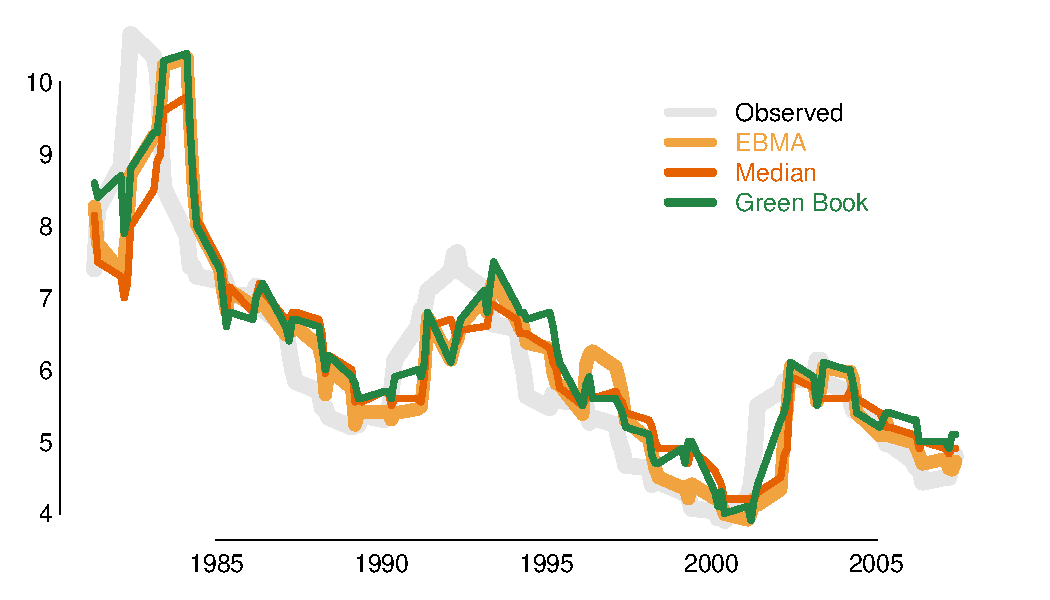
\includegraphics[scale=.8]{mdwtimeSeries2}
\end{center}
\end{figure}


Another approach to evaluating the performance of EBMA is to compare
its predictive accuracy to that made by other systematic forecasting
efforts and methods of generating ensemble predictions.  Specifically,
we compare EBMA's predictive accuracy to (1) the Green Book, (2) the
median forecaster prediction and (3) the mean forecaster
prediction.\footnote{Note that the EBMA model is calculated on only a the
  subset of forecasts that have made a sufficiently large number of
  recent predictions to calibrate model weights.  Thus, the median
  forecast and the ensemble forecast will not be the same even when
  $c=1$.  }  The first three of these forecasts and the true level of
unemployment are shown in Figure \ref{timeSeries}.

Figure \ref{timeSeries} shows a visual representation of the
Greenbook, median SPF and the EBMA (with $c=0.05$) forecasts over
time, as well as the true unemployment rate. As was noted above and is
clearly visible, the SPF and Greenbook forecasts are quite
similar. \citet{Baghestani:2008} noted that the Greenbook forecast is
slightly biased to over predict the unemployment rate. In some periods
EBMA is able to correct this bias, however given the similarity of
component models, the improvement in that direction is rather
small. In general, however, it is easily visible that the EBMA forecast
is closer to the actual rate than the median SPF or the Green Book
forecast.



\begin{table}[h]
\caption{Comparing adjusted EBMA models with Green Book, median, and mean forecasts of U.S. Unemployment (1981-2007)}
\begin{center}
\begin{tabular}{lrrrrrrrr}
\toprule
 & MAE & RMSE & MAD & RMSLE & MAPE & MEAPE & MRAE & PW \\ 
\midrule
 EBMA (c=0)& 0.54 & 0.74 & 0.37 & 0.093 & 8.37 & 6.49 & \textbf{0.73} & \textbf{27.36} \\ 
  EBMA (c=0.05)& \textbf{0.54} & 0.74 &\textbf{ 0.37} & \textbf{0.093} & \textbf{8.33} & \textbf{6.30} & 0.75 & \textbf{27.36} \\ 
 EBMA (c=0.1)& 0.54 & 0.74 & 0.35 & 0.093 & 8.40 & 6.44 & 0.76 & 28.30 \\ 
EBMA (c=1) & 0.61 & 0.80 & 0.46 & 0.102 & 9.72 & 8.92 & 0.95 & 46.23 \\ 
 Green Book& 0.57 & \textbf{0.73} & 0.43 & 0.093 & 9.37 & 8.81 & 1.00 & 45.28 \\ 
 Forecast Median& 0.62 & 0.81 & 0.47 & 0.103 & 9.83 & 8.87 & 0.98 & 47.17 \\ 
Forecast Mean& 0.61 & 0.80 & 0.46 & 0.102 & 9.71 & 9.06 & 0.93 & 46.23 \\ 
\bottomrule
\end{tabular}
\end{center}

\label{compareTable1}
Definitions of model fit statistics are provided in the Appendix. The model with the lowest score for each metric are shown in bold.  Differences between model performance may not be obvious due to rounding.
\end{table}


Table \ref{compareTable1} formally compares these baseline models
using all eight of the metrics to EBMA models with $c=$0, 0.05, 0.1,
and 1 respectively.  The bolded cells in each column indicate the
model that performed ``best'' as measured by each metric.  With one
exception, (the Green Book outperforms the ensemble by 0.01 on RMSE),
the EBMA model outperforms both the Green Book forecast and the
unweighted mean and median forecast on every metric.  Moreover, these
results indicate that the $c$ parameter is best set to a small number.
In general, the model with $c=0.05$ performs best (or is tied for
best) on six out of eight of these metrics.




\subsection{U.S. presidential elections}

Informed by the above discussion, we now turn to our second
application and return briefly to the example with which we began --
predicting U.S. presidential elections.  Using the forecasts shown in
Table 1, we fit an EBMA model with $c=0.05$.  The model weights and
in-sample fit statistics for the ensemble and its components are shown
in Table \ref{presModel}.


% latex table generated in R 2.15.1 by xtable 1.7-0 package
% Sun Aug 12 21:58:55 2012
\begin{table}[ht]
\caption{Model weights and in-sample fit statistics for EBMA model of U.S. Presidential Elections (1992-2008)}
\label{presModel}
\begin{center}
\begin{tabular}{lrrrr}
  \toprule
 & \shortstack{EBMA\\ Weight}&RMSE &MAE \\ 
  \midrule
EBMA &  & 1.92 & 1.56 \\ 
  Fair & 0.02 & 5.53 & 4.58 \\ 
  Abramowitz & 0.78 & 2.02 & 1.72 \\ 
  Campbell  & 0.07 & 3.46 & 2.88 \\ 
  Hibbs  & 0.04 & 2.68 & 2.44 \\ 
  Lewis-Beck, Rice, and Tien & 0.06 & 2.78 & 2.28 \\ 
  Lockerbie  & 0.00 & 7.33 & 6.97 \\ 
 Holbrook & 0.01 & 5.73 & 4.77 \\ 
  Erikson and Wlezien & 0.02 & 2.74 & 2.25 \\ 
  Cuz\`an & 0.00 & 1.27 & 0.95 \\ 
   \bottomrule
\end{tabular}
\end{center}
\end{table}

As can be seen in Table \ref{presModel}, the EBMA model assigns the
majority of weight to the Abramowitz model with the model by Campbell
receiving the second largest weight. These weights are based on the
performance of each model in forecasting the incumbent vote share in
the presidential elections between 1992 and 2008. The Cuz\`an and
Bundrick model is weighted to such a small degree because only
out-of-sample predictions for 2004 and 2008 were available here.




Figure \ref{pres} shows the posterior predictive distribution for the
2008 election (top) and, based on current forecasts from each of the
component models, the 2012 election.  We predict that Obama is going to
win by very little, however the credible intervals are quite wide,
indicating a lot of uncertainty. Component models predictive
distributions are shown in color (scaled by their respective weight),
while the EBMA predictive distribution is shown in black. Vertical
dashes indicate the point prediction of each model (bold dash for the
EBMA model). The vertical dashed line in the top panel depicts the
actual election result in 2008.

\begin{figure}[h]
\caption{Predictive ensemble PDFs of incumbent-part vote share in U.S. Presidential Elections}
\label{pres}
\begin{center}
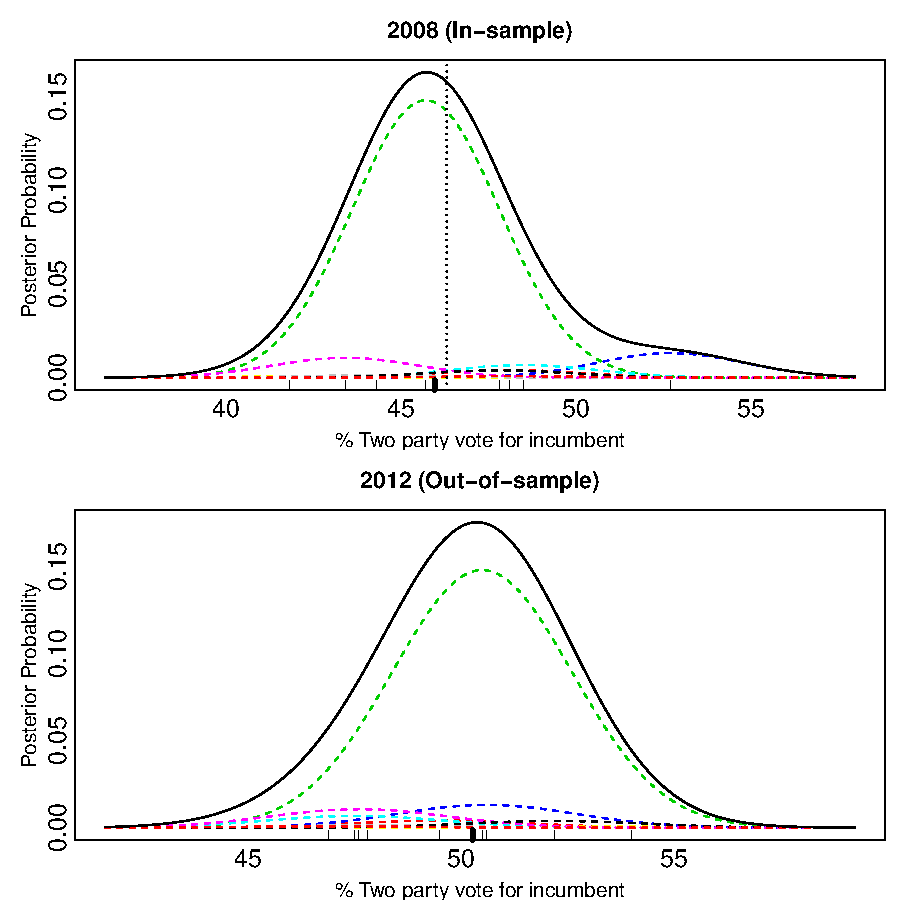
\includegraphics[scale=.8]{presForecast}
\end{center}
The figure shows the density functions for each of the component
models in different colors and scaled by their respective weight. The
point predictions of the individual models are depicted by smalls
vertical dashes. The black curve is the density of the EBMA
prediction, with the bold dash indicating the EBMA point
prediction. For 2008 the vertical dashed line shows the actual result.
\end{figure}


\section{Discussion} 

Ensemble Bayesian model averaging is a principled way of combining
forecasts to improve prediction accuracy. However, the calibration of
such models in the social sciences is often hindered by the quality as
well as availability of data. For one, in many forecasting exercises
the number of forecasting models is large, yet the number of
observations on which the EBMA model can be trained is small. This
creates problems for the estimation of model weights, as it is likely
that overly high weights are assigned to models that are performing
well over this particular period. This is especially true should the
EBMA model be calibrated on in-sample forecasts of the component
models. Second, many predictive models do not provide forecasts for
all observations in the sample, as some forecasts may be missing or
the time-periods for which forecasts were made are different for
different models. In the standard EBMA model introduced in
\citet{mhw:2012} missing observations in component model predictions
are not allowed.


In this manuscript, we address both of these issues to make
EBMA more applicable for researchers and so-called predictioneers in the social
sciences. After reviewing the standard EBMA framework, we proceed to
introduce an adjustment to the EBMA estimation that allows for missing
observations in the calibration period. As a further adjustment, we
then propose to introduce a ``wisdom of the crowds'' parameter into
the model, which forces EBMA to put some minimal weight on all
component models. Adding this constant aids the calibration of EBMA
when the number of observations in the calibration period is small.

After explaining our adjustments, we apply the adjusted EBMA model in
two prediction exercises. In Section \ref{econ}, we use ensemble
Bayesian model averaging to combine predictions of the unemployment
rate in the US from the Survey of Professional Forecasters as well as
the Green Book. As we show, even when a large number of forecasts is
missing for any given quarter, EBMA generally outperforms the
Green Book, SPF component models, as well as the median and mean SPF
forecast. 

In a second example, we use the out-of-sample forecasts of nine
prediction models of presidential elections from 1992 to 2008 to
calibrate an ensemble model. We use the model calibrated to make an
informed prediction for the 2012 elections based on a weighted
combination of the component model predictions for 2012. According to
the EBMA model, we expect President Obama to win the popular vote in
the 2012 election by a small margin (the uncertainty estimated around
the prediction is quite large).

% Missing data is always a conundrum, and a pain. This is especially
% true when creating ensemble predictions. The combination of missing
% observations with short calibration periods is especially
% damaging. EBMA typically underweights the ensembles with a lot of
% missing observations, and as a result can diminish, rather than
% enhance, the predictive accuracy of the weighted average. We introduce
% a way around this problem by the introduction of a parameter which
% spreads the weights out over the ensemble components in a way that
% helps to preserve the advantages of the ensemble.

Finally, we note that in future drafts of this paper, we hope to (1)
compare alternative methods of handling missing data (2) discuss how
to select window of time for calibration and (3) conduct some
simulation studies to explore settings for $c$ parameter and to test
the numerical stability of our results.


% JACOB, statisticians will want to know why we don't just estimate C.
% MIKE, we probably could in a fully Bayesian framework.  But to
% identify the model, we would still probably have to put bounds on it.


 \newpage
 \appendix


 \section*{Predictive Metrics Appendix}

 Denote the forecast of observation $i$ as $f_i$ and the observed
 outcome as $y_i$.  We define the \textit{absolute error} as
 $e_i\equiv |f_i - y_i|$ and the \textit{absolute percentage error} as
 $a_i \equiv e_i / |y_i| \times 100$.  Finally, for each observation we have
 prediction from naive forecast, $r_i$, that serves as a baseline for
 comparison.  In the example is the main text, this naive model is
 simply the lagged observation.  We can therefore define $b_i \equiv
 |r_i - y_i|$.\footnote{See \citet{brandt:freeman:schrodt:2011} for
   additional discussion of comparative fit metrics.}

 Donating the median of some vector $\mathbf{x}$ as $med(\mathbf{x})$,
 and the standard indicator function as $I(.)$, we define the following heuristic statistics:
 \begin{eqnarray*}
 \mathrm{MAE} &=& \frac{\sum_1^n{e_i}}{n}\\
  \mathrm{RMSE} &=& \sqrt{\frac{\sum_1^n{e^2_i}}{n}} \\
  \mathrm{MAD} &=& \mathrm{med}(\mathbf{e}) \\
  \mathrm{RMSLE} &=& \sqrt{\frac{\sum_1^n\left(ln(f_i+1) - ln(y_i+1)  \right)^2}{n}} \\
  \mathrm{MAPE} &=& \frac{\sum_1^n{a_i}}{n} \\
   \mathrm{MEAPE} &=& \mathrm{med}(\mathbf{a}) \\
 \mathrm{MRAE} &=& \mathrm{med}\left(\frac{e_1}{b_1}, \ldots, \frac{e_n}{b_n} \right) \\
 \mathrm{PW} &=& \frac{\sum_1^nI(e_i > b_i)}{n} \times 100
\end{eqnarray*}



%%Bib 
\singlespacing
\bibliographystyle{apsr}
\bibliography{Bibliography_EBMA}


\end{document}
\bye
